\documentclass[11pt]{article}
\usepackage[a4paper,margin=2.25cm]{geometry}
\usepackage[T1]{fontenc}
\usepackage[utf8]{inputenc}
\usepackage{lmodern}
\usepackage{amsmath,mathtools}
\usepackage{graphicx}
\usepackage{booktabs,tabularx,array}
\usepackage{microtype}
\usepackage{caption}
\usepackage{float}
\usepackage[hidelinks]{hyperref}
\hypersetup{
  pdftitle={Online Resource 1 - finite-population ABM benchmark and event-level verification},
  pdfauthor={Seyfullah Enes Kotil},
  pdfsubject={Supplementary methods, numerical comparisons, and direct event-level verification},
  pdfkeywords={contact tracing, agent-based model, deterministic hierarchy, event-level verification}
}
\usepackage{fancyhdr}
\usepackage{lastpage}
\setlength{\parindent}{0pt}
\setlength{\parskip}{0.58em}
\setlength{\emergencystretch}{3em}
\renewcommand{\arraystretch}{1.12}
\renewcommand{\thefigure}{OR1.\arabic{figure}}
\renewcommand{\thetable}{OR1.\arabic{table}}
\captionsetup[figure]{name=Fig.,font=small,labelfont=bf,labelsep=space,justification=justified,singlelinecheck=false}
\captionsetup[table]{font=small,labelfont=bf,labelsep=space,justification=justified,singlelinecheck=false,position=top}
\pagestyle{fancy}
\fancyhf{}
\fancyhead[L]{\small Online Resource 1}
\fancyhead[R]{\small Kotil}
\fancyfoot[C]{\small \thepage\ of \pageref{LastPage}}
\setlength{\headheight}{14pt}
\begin{document}
\pdfbookmark[0]{Online Resource 1}{or1-cover}
\begin{center}
{\Large\bfseries Online Resource 1: Supplementary Information}\\[1.0em]
{\large\bfseries Overlapping roots: a transmission-tree framework for population-level contact-tracing dynamics}\\[1.2em]
{\bfseries Journal:} Bulletin of Mathematical Biology\\[0.5em]
{\bfseries Author:} Seyfullah Enes Kotil\\[0.4em]
Boğaziçi University, Department of Molecular Biology and Genetics, Istanbul, Türkiye\\
Bahçeşehir University, School of Medicine, Department of Biophysics, Istanbul, Türkiye\\[0.5em]
{\bfseries Corresponding author:} enesseyfullah.kotil@bogazici.edu.tr\\[1.2em]
{\bfseries Online Resource 1}\\
Supplementary methods, figures, and numerical comparison of the finite-population ABM and deterministic hierarchy, including direct event-level verification
\end{center}
\vspace{0.5em}\hrule\vspace{1em}

\textbf{Associated supplementary files.} Online Resource 2 (\texttt{ESM\_2.xlsx}) contains all 780 dimensional parameterizations, the published trajectory-error and convergence summaries, and deterministic-reference and event-term checks. Online Resource 3 (\texttt{ESM\_3.zip}) contains the available executable and audit code, numerical tables and data, event-term verification data, figure-generation files, and software requirements.

\section*{OR1-S1 Finite-population agent-based benchmark}
\pdfbookmark[1]{OR1-S1 Finite-population agent-based benchmark}{or1-s1}
The finite-population agent-based model (ABM) simulates transmission, spontaneous removal, detection, and instantaneous one-step forward tracing on the active transmission forest. Individual identities and unique infector--infectee links are retained throughout each realization. Let $S^{\mathrm{ABM}}(t)$ and $I^{\mathrm{ABM}}(t)$ denote the susceptible and infectious counts in physical time. Transmission, spontaneous removal, and detection occur at total rates
\[
\beta S^{\mathrm{ABM}}(t)I^{\mathrm{ABM}}(t),\qquad
\gamma I^{\mathrm{ABM}}(t),\qquad
\gamma_c I^{\mathrm{ABM}}(t),
\]
respectively. At transmission, an infectious individual is selected uniformly as the infector, one susceptible individual becomes infectious, and the new case is recorded as an active child of its infector. At spontaneous removal, the selected individual leaves the active infectious set. At detection, the selected individual is removed and each active direct infectee is independently removed with probability $p_f$; traced removals do not initiate further tracing. Descendant-depth observables $M_k^{\mathrm{ABM}}(t)$ can be computed directly from the active transmission forest at each observation time; the numerical trajectory comparison uses $M_1^{\mathrm{ABM}}$. The process is simulated with an exact event-driven Gillespie algorithm.

The dimensional parameters determine
\[
\Gamma=\gamma+\gamma_c,\qquad
\tau=\Gamma t,\qquad
R=\frac{\beta S_0}{\Gamma},\qquad
c=\frac{\gamma_c p_f}{\Gamma}.
\]
The process is simulated in physical time and reported on $0\leq\tau\leq5$. Detection operates throughout the comparison experiments, whereas forward tracing is activated at $\tau_{\mathrm{on}}=0.5$. The same activation schedule is imposed in the deterministic reference.

\section*{OR1-S2 Crossed dimensional parameterizations}
\pdfbookmark[1]{OR1-S2 Crossed dimensional parameterizations}{or1-s2}
The nondimensional parameters $R$ and $c$ do not uniquely determine the dimensional rates. We therefore cross
\[
\Gamma\in\left\{\frac14,\frac12,1,2,4\right\}
\]
with three explicit detection--tracing decompositions. For prescribed $R$, $c$, $S_0$, and $\Gamma$, the parameterizations are
\begin{table}[H]
\caption{Crossed dimensional parameterizations for $0\leq c<1$}
\centering\small
\begin{tabularx}{\textwidth}{@{}p{0.34\textwidth}cccc@{}}
\toprule
Decomposition & $\beta$ & $\gamma$ & $\gamma_c$ & $p_f$ \\
\midrule
Less-frequent detection, complete tracing & $R\Gamma/S_0$ & $\Gamma(1-c)$ & $\Gamma c$ & $1$ \\
Intermediate & $R\Gamma/S_0$ & $\Gamma(1-c)/2$ & $\Gamma(1+c)/2$ & $2c/(1+c)$ \\
Frequent detection, partial tracing & $R\Gamma/S_0$ & $0$ & $\Gamma$ & $c$ \\
\bottomrule
\end{tabularx}
\end{table}
Every row satisfies
\[
\gamma+\gamma_c=\Gamma,\qquad
\frac{\beta S_0}{\Gamma}=R,\qquad
\frac{\gamma_c p_f}{\Gamma}=c.
\]
At $c=1$, the three rows coincide, and one parameterization is retained for each value of $\Gamma$. At $c=0$, the three rows differ in the labeling of primary removal, but no tracing removal occurs.

The analysis uses $R\in\{2,4,6\}$ and $c\in\{0,0.25,0.5,0.75,1\}$. For each population scale, this gives 195 raw-rate protocols: 65 for each value of $R$. All raw-rate protocols are simulated directly. For $S_0\in\{500,1000,2000\}$, one independent pool of 120 trajectories is generated per protocol for population-size convergence. At $S_0=8000$, 30 independent pools of 120 trajectories are generated for every protocol; the first prespecified pool (pool 0) is also used as the $S_0=8000$ point in the population-size comparison. The 30 pools give
\[
195\times30\times120=702{,}000
\]
ABM trajectories at the selected population scale.

\begin{table}[H]
\caption{Global numerical settings}
\centering\small
\begin{tabularx}{\textwidth}{@{}p{0.34\textwidth}X@{}}
\toprule
Setting & Value \\
\midrule
Nondimensional grid & $R\in\{2,4,6\}$, $c\in\{0,0.25,0.5,0.75,1\}$ \\
Dimensional rate scales & $\Gamma\in\{1/4,1/2,1,2,4\}$ \\
Population scales & $S_0\in\{500,1000,2000,8000\}$, $I_0=0.02S_0$ \\
Raw-rate protocols & 195 per population scale; 780 parameterizations in total \\
Population convergence & One 120-realization pool per protocol; at $S_0=8000$, pool 0 of the 30 replicate-convergence pools is used \\
Replicate convergence at $S_0=8000$ & 30 independent 120-realization pools per raw-rate protocol \\
Observation grid & 151 equally spaced points on $0\leq\tau\leq5$ \\
Tracing activation & $\tau_{\mathrm{on}}=0.5$ \\
High-depth reference & $K_{\mathrm{ref}}=40$, checked against $K=80$ \\
Deterministic solver & BDF; relative tolerance $10^{-10}$, absolute tolerance $10^{-12}$, maximum step $0.025$ \\
Pointwise confidence intervals & Normal approximation; conditional on $I(\tau)>0$ for $m_1$ \\
Master seed & 20260804 \\
\bottomrule
\end{tabularx}
\end{table}

\section*{OR1-S3 High-depth deterministic reference}
\pdfbookmark[1]{OR1-S3 High-depth deterministic reference}{or1-s3}
For each $(R,c)$, the ABM ensemble mean is compared with a high-depth numerical solution retaining $S$, $I$, and $M_1,\ldots,M_{K_{\mathrm{ref}}}$, with $K_{\mathrm{ref}}=40$. The initial state is
\[
S(0)=S_0,\qquad I(0)=I_0,\qquad M_k(0)=0\quad(k\geq1).
\]
At the terminal retained level, $M_{K_{\mathrm{ref}}+1}=0$ is imposed. High-depth trajectories are computed with the BDF method using relative tolerance $10^{-10}$, absolute tolerance $10^{-12}$, and maximum dimensionless step size $0.025$. The intervals before and after $\tau_{\mathrm{on}}=0.5$ are integrated separately so that the change in the tracing terms is imposed exactly at the activation time. The structural bound $0\leq M_{K_{\mathrm{ref}}+1}\leq M_{K_{\mathrm{ref}}}$ follows from Lemma 1 of the main manuscript, but adequacy is assessed independently by repeating the calculation with $K=80$. Across the full grid and observation interval, the maximum absolute difference in $(S/S_0,I/S_0,M_1/S_0)$ was $2.99\times10^{-10}$.

\section*{OR1-S4 Ensemble-mean trajectory error and convergence}
\pdfbookmark[1]{OR1-S4 Ensemble-mean trajectory error and convergence}{or1-s4}
For realization $\ell$, define
\[
\mathbf z^{\mathrm{ABM},(\ell)}(\tau)=\left(\frac{S^{\mathrm{ABM},(\ell)}}{S_0},\frac{I^{\mathrm{ABM},(\ell)}}{S_0},\frac{M_1^{\mathrm{ABM},(\ell)}}{S_0}\right).
\]
For a pool of $n$ independent realizations, $\overline{\mathbf z}_n^{\mathrm{ABM}}=n^{-1}\sum_{\ell=1}^n\mathbf z^{\mathrm{ABM},(\ell)}$. With $\mathbf z^{\mathrm{HD}}$ denoting the high-depth trajectory,
\[
E_{\mathrm{mean}}=\left[\frac1T\int_0^T\left\|\overline{\mathbf z}_n^{\mathrm{ABM}}(\tau)-\mathbf z^{\mathrm{HD}}(\tau)\right\|_2^2\,\mathrm d\tau\right]^{1/2}.
\]
The integral is evaluated over $0\leq\tau\leq5$ at 151 equally spaced observation times using the trapezoidal rule. Extinct realizations remain at $I^{\mathrm{ABM}}=M_1^{\mathrm{ABM}}=0$ and contribute to unconditional scaled-count means. Pointwise 95\% confidence intervals in Figs.~\ref{fig:s2} and~\ref{fig:s3} are calculated as $\overline{x}(\tau)\pm1.96s_x(\tau)/\sqrt{n_\tau}$. For $S$, $I$, and $M_1$, $n_\tau=120$. For $m_1=M_1/I$, the mean, standard deviation, and confidence interval are calculated conditionally over realizations satisfying $I(\tau)>0$, and $n_\tau$ is the number of contributing nonextinct realizations.

For population-size convergence, one 120-realization pool is used for each raw-rate protocol. For $S_0\in\{500,1000,2000\}$, this pool is generated independently for the population-size calculation. At $S_0=8000$, the first prespecified pool (pool 0) among the 30 pools generated for replicate convergence is reused in the population-size comparison. For replicate convergence at $S_0=8000$, every raw-rate protocol has 30 independent master pools. Within each pool, the 120 trajectories are randomly permuted once, and the first $n$ trajectories are used for $n\in\{1,2,5,10,20,40,80,120\}$. Thus, each value of $n$, including $n=120$, has
\[
195\times30=5850
\]
independent ensemble-error estimates. Estimates at different values of $n$ are paired within a pool, but the 5850 estimates at any fixed $n$ arise from independent pools. The representative trajectory plots in Figs.~\ref{fig:s2}--\ref{fig:s4} use the first prespecified independently generated pool (pool 0) for each displayed protocol; no pool was selected according to its agreement with the deterministic reference.

\begin{table}[H]
\caption{Population-size convergence. Each row summarizes one 120-realization ensemble for each of the 195 raw-rate protocols. For $S_0=8000$, the first prespecified pool (pool 0) among the 30 independently generated pools is used.}
\centering\footnotesize
\begin{tabular}{@{}rrrrrrr@{}}
\toprule
$S_0$ & $I_0$ & Protocols & Estimates & Median & 10th percentile & 90th percentile \\
\midrule
500 & 10 & 195 & 195 & 0.012926 & 0.006713 & 0.026509 \\
1000 & 20 & 195 & 195 & 0.006759 & 0.002899 & 0.013034 \\
2000 & 40 & 195 & 195 & 0.003335 & 0.001572 & 0.006732 \\
8000 & 160 & 195 & 195 & 0.001337 & 0.000664 & 0.002717 \\
\bottomrule
\end{tabular}
\end{table}

\begin{table}[H]
\caption{Replicate convergence at $S_0=8000$. Thirty independent 120-realization pools were generated for each of the 195 raw-rate protocols. Consequently, every value of $n$, including $n=120$, is summarized by 5850 independent ensemble-error estimates.}
\centering\footnotesize
\begin{tabular}{@{}rrrrrrr@{}}
\toprule
$n$ & Protocols & Pools/protocol & Estimates & Median & 10th percentile & 90th percentile \\
\midrule
1 & 195 & 30 & 5850 & 0.012499 & 0.006548 & 0.027396 \\
2 & 195 & 30 & 5850 & 0.008872 & 0.004631 & 0.019258 \\
5 & 195 & 30 & 5850 & 0.005733 & 0.002934 & 0.012062 \\
10 & 195 & 30 & 5850 & 0.003970 & 0.002051 & 0.008892 \\
20 & 195 & 30 & 5850 & 0.002852 & 0.001492 & 0.006218 \\
40 & 195 & 30 & 5850 & 0.002062 & 0.001051 & 0.004493 \\
80 & 195 & 30 & 5850 & 0.001532 & 0.000775 & 0.003413 \\
120 & 195 & 30 & 5850 & 0.001308 & 0.000654 & 0.002885 \\
\bottomrule
\end{tabular}
\end{table}

\section*{OR1-S5 Supplementary numerical results}
\pdfbookmark[1]{OR1-S5 Supplementary numerical results}{or1-s5}
Population-size convergence was systematic: increasing $S_0$ from 500 to 8000 reduced the median ensemble-mean trajectory error from 0.012926 to 0.001337, with a descriptive log--log slope of -0.82 over the tested population scales. On this basis, $S_0=8000$ was selected as the finite-population benchmark. It was the largest population examined, yielded discrepancies of order $10^{-3}$, and remained computationally feasible for the full crossed parameter design. This is an empirically supported working scale rather than a universal threshold, and the reported discrepancies are empirical summaries rather than rigorous error bounds.

At $S_0=8000$, $I_0=160$, and $n=120$, the 5850 independently generated ensembles had median trajectory error 0.001308, mean 0.001578, 90th percentile 0.002885, and maximum 0.006918. The descriptive log--log slope with replicate count was -0.48, close to the $n^{-1/2}$ reference scaling.

\begin{table}[H]
\caption{Trajectory-error summary by nondimensional grid cell at $S_0=8000$ and $n=120$. Each raw-rate protocol contributes 30 independently generated ensembles.}
\centering\scriptsize
\begin{tabular}{@{}rrrrrrrr@{}}
\toprule
$R$ & $c$ & Protocols & Estimates & Median & Mean & 90th percentile & Maximum \\
\midrule
2 & 0 & 15 & 450 & 0.001786 & 0.002104 & 0.003983 & 0.006454 \\
2 & 0.25 & 15 & 450 & 0.002028 & 0.002302 & 0.004118 & 0.006816 \\
2 & 0.5 & 15 & 450 & 0.001761 & 0.002100 & 0.003910 & 0.006918 \\
2 & 0.75 & 15 & 450 & 0.001658 & 0.001950 & 0.003545 & 0.006671 \\
2 & 1 & 5 & 150 & 0.001613 & 0.001772 & 0.003014 & 0.005445 \\
4 & 0 & 15 & 450 & 0.001225 & 0.001402 & 0.002466 & 0.004225 \\
4 & 0.25 & 15 & 450 & 0.001294 & 0.001479 & 0.002607 & 0.004766 \\
4 & 0.5 & 15 & 450 & 0.001303 & 0.001502 & 0.002474 & 0.004674 \\
4 & 0.75 & 15 & 450 & 0.001368 & 0.001538 & 0.002493 & 0.006012 \\
4 & 1 & 5 & 150 & 0.001545 & 0.001730 & 0.002964 & 0.004726 \\
6 & 0 & 15 & 450 & 0.000992 & 0.001136 & 0.001870 & 0.003310 \\
6 & 0.25 & 15 & 450 & 0.001012 & 0.001132 & 0.001950 & 0.003527 \\
6 & 0.5 & 15 & 450 & 0.000995 & 0.001146 & 0.001988 & 0.003897 \\
6 & 0.75 & 15 & 450 & 0.001006 & 0.001174 & 0.001999 & 0.003481 \\
6 & 1 & 5 & 150 & 0.001046 & 0.001148 & 0.001792 & 0.003065 \\
\bottomrule
\end{tabular}
\end{table}

\begin{figure}[H]
\centering
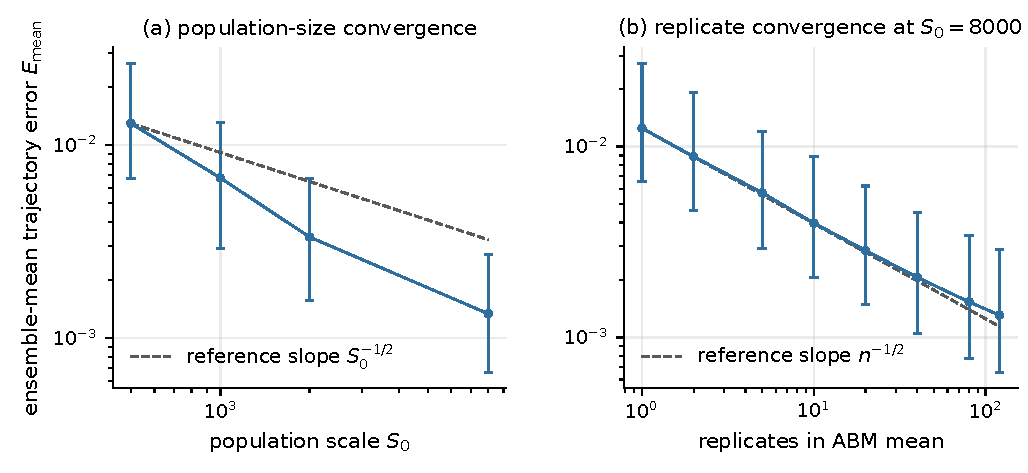
\includegraphics[width=\textwidth]{figures/supp_S1_convergence_U8000.pdf}
\caption{Convergence of the ABM ensemble-mean trajectory error. Panel (a) summarizes one 120-realization ensemble for each of 195 raw-rate protocols at each population scale; for $S_0=8000$, this is the first prespecified pool (pool 0) among the 30 independently generated pools. Panel (b) uses 30 independent pools per protocol at $S_0=8000$, yielding 5850 estimates for every $n$, including $n=120$. Points show medians and error bars the 10th and 90th percentiles. Dashed lines indicate $S_0^{-1/2}$ and $n^{-1/2}$ reference scalings.}
\label{fig:s1}
\end{figure}

\begin{table}[H]
\caption{Representative frequent-detection, partial-tracing errors shown in Fig.~\ref{fig:s2}}
\centering\small
\begin{tabular}{@{}rrrrr@{}}
\toprule
$c$ & $E_S$ & $E_I$ & $E_{M_1}$ & $E_{\mathrm{mean}}$ \\
\midrule
0 & 0.000722 & 0.000775 & 0.000586 & 0.001211 \\
0.25 & 0.003258 & 0.001966 & 0.001638 & 0.004143 \\
0.5 & 0.000898 & 0.000837 & 0.000900 & 0.001522 \\
0.75 & 0.000602 & 0.000350 & 0.000313 & 0.000763 \\
1 & 0.002752 & 0.001310 & 0.001063 & 0.003228 \\
\bottomrule
\end{tabular}
\end{table}

\begin{figure}[H]
\centering
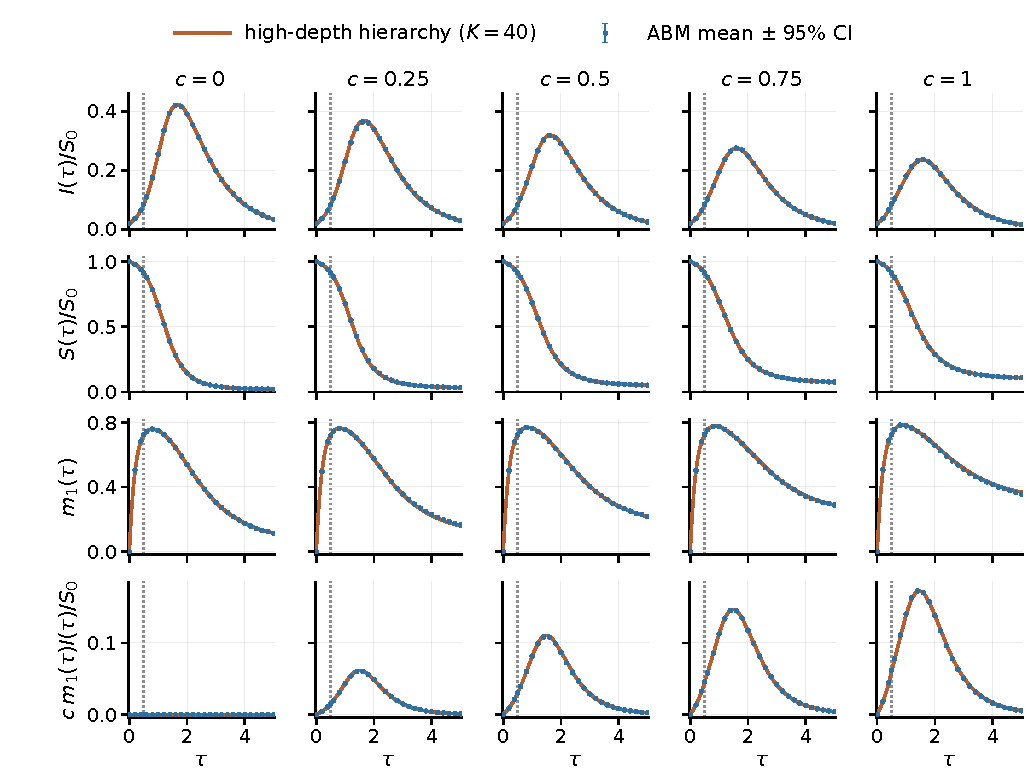
\includegraphics[width=\textwidth]{figures/supp_S2_selected_production_validation_U8000.pdf}
\caption{Finite-population ABM--hierarchy comparison at $R=4$, $S_0=8000$, $I_0=160$, and 120 realizations. The representative protocol uses $\Gamma=1$ and frequent detection with partial tracing. The first prespecified independently generated pool is shown. Points are ABM means with pointwise normal-approximation 95\% confidence intervals, solid curves are the $K=40$ hierarchy, and the vertical dotted line marks tracing activation at $\tau=0.5$. The $m_1$ summaries are conditional on $I(\tau)>0$.}
\label{fig:s2}
\end{figure}

\begin{table}[H]
\caption{Matched decomposition errors shown in Fig.~\ref{fig:s3}}
\centering\small
\begin{tabular}{@{}lrrrrr@{}}
\toprule
Protocol & $\Gamma$ & $E_S$ & $E_I$ & $E_{M_1}$ & $E_{\mathrm{mean}}$ \\
\midrule
Frequent partial & 1 & 0.000898 & 0.000837 & 0.000900 & 0.001522 \\
Less-frequent complete & 1 & 0.001840 & 0.001109 & 0.000833 & 0.002304 \\
\bottomrule
\end{tabular}
\end{table}

\begin{figure}[H]
\centering
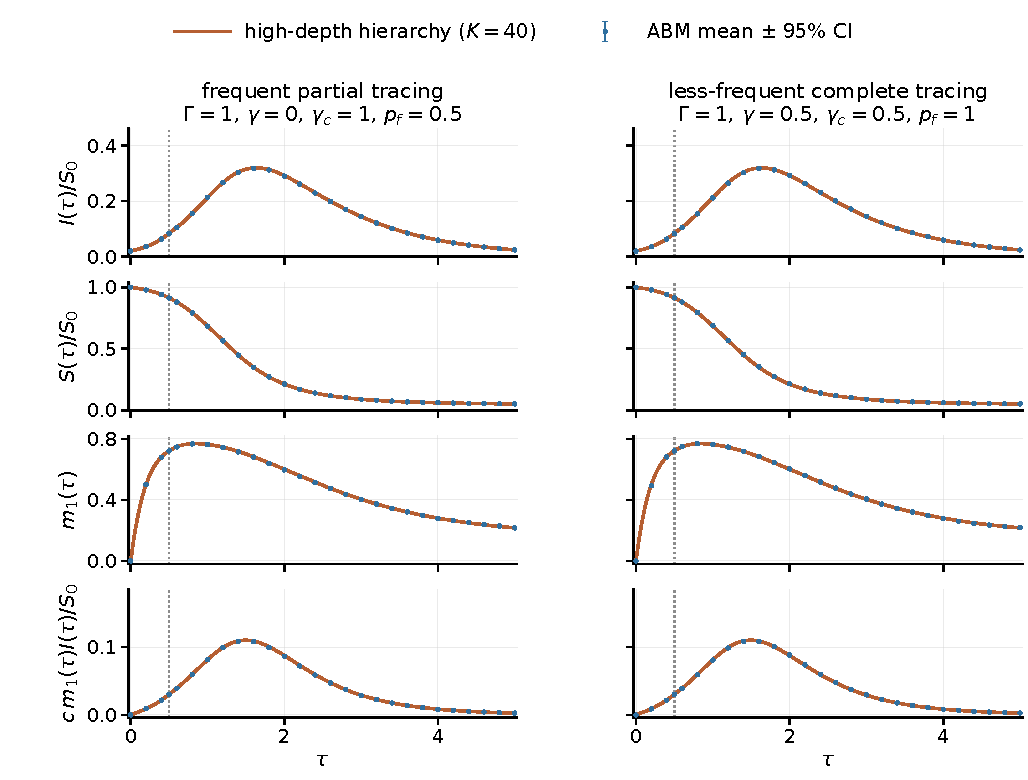
\includegraphics[width=\textwidth]{figures/supp_S3_matched_c_raw_rate_comparison_U8000.pdf}
\caption{Alternative detection--tracing decompositions at $R=4$, $c=0.5$, and $\Gamma=1$. Both protocols share the same nondimensional deterministic reference but differ in detection frequency and tracing probability. The first prespecified independently generated pool is shown for each protocol. Points are ABM means with pointwise normal-approximation 95\% confidence intervals; the $m_1$ summaries are conditional on $I(\tau)>0$.}
\label{fig:s3}
\end{figure}

\begin{table}[H]
\caption{Directly simulated rate-scale protocols shown in Fig.~\ref{fig:s4}}
\centering\small
\begin{tabular}{@{}rrrrrr@{}}
\toprule
$\Gamma$ & $\beta$ & $\gamma$ & $\gamma_c$ & $p_f$ & $E_{\mathrm{mean}}$ \\
\midrule
0.25 & 0.0001250 & 0 & 0.25 & 0.5 & 0.000723 \\
0.5 & 0.0002500 & 0 & 0.5 & 0.5 & 0.000936 \\
1 & 0.0005000 & 0 & 1 & 0.5 & 0.001522 \\
2 & 0.0010000 & 0 & 2 & 0.5 & 0.001686 \\
4 & 0.0020000 & 0 & 4 & 0.5 & 0.001132 \\
\bottomrule
\end{tabular}
\end{table}

\begin{figure}[H]
\centering
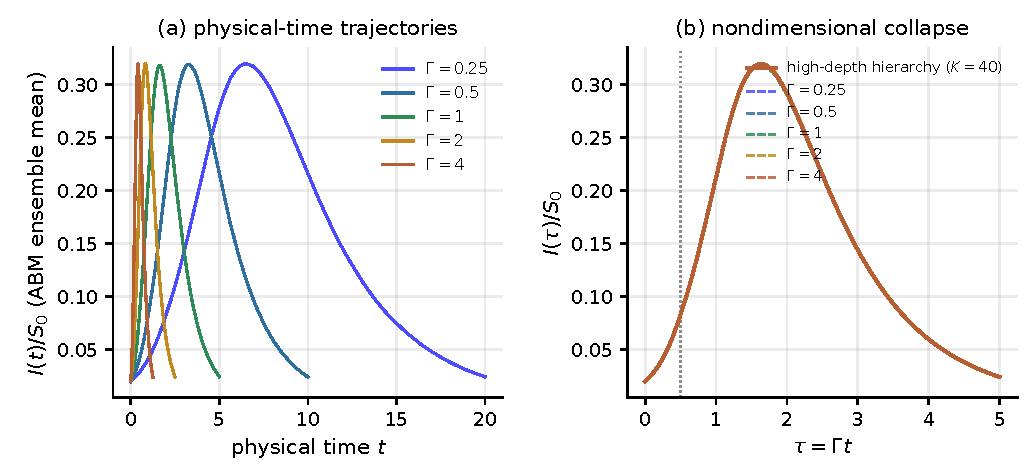
\includegraphics[width=\textwidth]{figures/supp_S4_rate_scale_collapse_U8000.pdf}
\caption{Direct simulation of dimensional rate rescaling. Independently generated 120-realization ABM ensembles are shown for $\Gamma\in\{1/4,1/2,1,2,4\}$ at $R=4$ and $c=0.5$. The first prespecified pool is used for each rate scale. Panel (a) shows physical-time trajectories over $0\leq t\leq5/\Gamma$; proportional changes in the dimensional event rates alter the physical time scale. Panel (b) shows the same ABM ensemble means in $\tau=\Gamma t$, where they collapse closely onto the common high-depth reference. This is an implementation and nondimensionalization check rather than an additional biological sensitivity analysis.}
\label{fig:s4}
\end{figure}

\section*{OR1-S6 Direct event-level verification of the balance terms}
\pdfbookmark[1]{OR1-S6 Direct event-level verification of the balance terms}{or1-s6}
The trajectory comparison tests the combined evolution of $S$, $I$, and $M_1$. To verify the individual balance terms directly, an instrumented version of the same event-driven ABM also records transmission events, spontaneous removals, case-identification events, and the number of infectious direct infectees removed through tracing. Traced removals are counted individually and occur as consequences of identification events; they do not constitute a separate Gillespie clock.

For realization $\ell$, the event intensities per unit dimensionless time are
\[
q_{\mathrm{trans}}^{(\ell)}=\frac{\beta}{\Gamma}S^{\mathrm{ABM},(\ell)}I^{\mathrm{ABM},(\ell)},
\qquad
q_{\mathrm{rec}}^{(\ell)}=\frac{\gamma}{\Gamma}I^{\mathrm{ABM},(\ell)},
\]
\[
q_{\mathrm{id}}^{(\ell)}=\frac{\gamma_c}{\Gamma}I^{\mathrm{ABM},(\ell)},
\qquad
q_{\mathrm{trace}}^{(\ell)}=
\mathbf 1_{\{\tau\geq\tau_{\mathrm{on}}\}}
\frac{\gamma_c p_f}{\Gamma}M_1^{\mathrm{ABM},(\ell)}.
\]
For each interval $B_j=[\tau_j,\tau_{j+1})$, the observed ensemble-mean count is $n^{-1}\sum_{\ell}\Delta N_{e,\ell j}$ and the state-supplied analytical expectation is $n^{-1}\sum_{\ell}\int_{B_j}q_e^{(\ell)}(\tau)\,\mathrm d\tau$. The state integrals are accumulated exactly over the piecewise-constant ABM holding intervals and are split at the observation boundaries and at $\tau_{\mathrm{on}}=0.5$. Thus, the analytical axis is formed from the measured ABM states on the same paths and does not use a deterministic reference trajectory or a midpoint approximation.

The analysis uses $S_0=8000$, $I_0=160$, the full set of 195 raw-rate protocols, and 120 independently generated realizations per protocol. The interval $0\leq\tau\leq5$ is divided into 150 equal bins. There are therefore 29,250 protocol--interval comparisons for transmission, spontaneous removal, and identification. The traced-removal panel contains 20,250 positive-hazard comparisons; 9000 zero-hazard intervals were verified separately, and none contained a traced removal.

The aggregate observed-to-expected ratios were 1.00002 for transmission, 1.00009 for spontaneous removal, 0.99997 for identification, and 1.00010 for traced removal.

The corresponding four-panel calibration scatter plot is shown as Figure~2 of the main text, together with the through-origin calibration slopes and coefficients of determination for each panel.

\section*{OR1-S7 Reproducibility files}
\pdfbookmark[1]{OR1-S7 Reproducibility files}{or1-s7}
Online Resources 2 and 3 provide the dimensional parameter table, published error and convergence summaries, deterministic-reference and event-term diagnostics, available executable and audit code, numerical and figure data, figure-generation files, and software requirements.
\end{document}
